%!TEX root=../../root.tex
\section{Lezione 21}

\subsection{La classe \emph{coNP}}

\subsubsection{Definizione}
\[
	\emph{coNP} = \left\{ \ L \ | \ \overline{L} \in NP \right\}
\]
Ossia \emph{coNP} contiene tutti i linguaggi il cui complemento è in NP. \\
La classe \emph{coNP} è interessante dal punto di vista teorico poiché dimostrare che \emph{coNP} sia diversa da NP equivarrebbe a dimostrare la diversità di P ed NP. \\

\begin{align*}
	P = NP &\implies NP = \emph{coNP} \\ 
	NP \neq \emph{coNP} &\implies P \neq NP
\end{align*} 

\subsubsection{\emph{coNP}-Completezza}
\newtheorem*{def1}{Definizione}
\begin{def1}
	L è \emph{coNP}-Completo se:
	\begin{enumerate}
		\item $L \in coNP$
		\item L è \emph{coNP-Hard}, ossia $\forall A \in coNP, A \leq_{p} L$
	\end{enumerate}
\end{def1}

\subsubsection{\texorpdfstring{Il problema $\overline{TAUT}$}{Il complemento di TAUT}}
\begin{gather*}
	TAUT = \left\{ \ \varphi \ | \ \varphi \ \text{è vera per ogni assegnamento} \ \right\} \\
	\overline{TAUT} = \left\{ \ \varphi \ | \ \exists \ \text{un assegnamento che rende} \ \varphi \ \text{falsa} \ \right\}
\end{gather*}
Dimostreremo ora che $TAUT$ è \emph{coNP-Completo}.
\newtheorem*{tautcoNP}{Teorema}
\begin{tautcoNP}
	$TAUT \in coNP$
\end{tautcoNP}
\begin{proof}[Dimostrazione]
Dobbiamo mostrare che $\overline{TAUT}$, il problema della falsificabilità di formule booleane, sta in $NP$. Siamo in grado di esibirne un algoritmo (i.e. una $NTM$) che lo decide: esso è analogo a quello che decide $SAT$, soltanto che invece di controllare che vi sia un assegnamento che soddisfi la formula si controlla che ve ne sia uno che la falsifichi. 
\end{proof}

\newtheorem*{tautcoNPhard}{Teorema}
\begin{tautcoNPhard}
	$TAUT$ è coNP-completo
\end{tautcoNPhard}
\begin{proof}[Dimostrazione]
Abbiamo mostrato prima che $\overline{TAUT} \in NP \implies TAUT \in coNP$; ci resta da mostrare che $TAUT$ sia $coNP$-hard.

Sappiamo che $\forall A \in NP \quad A \leq_{p} SAT$ poiché SAT è \emph{NP-Completo}, inoltre sappiamo che se un linguaggio A si riduce ad un linguaggio B allora anche il complemento di A si può ridurre al complemento di B, quindi $\overline{A} \leq_{p} \overline{SAT}$. \\
Basta quindi dimostrare che $\overline{SAT}$ si riduce polinomialmente a TAUT per dimostrare la \emph{coNP-Hardness} di quest'ultimo. Essendo le istanze sì di $\overline{SAT}$ le formule insoddisfacibili basterà associare ad ogni formula accettata da SAT la sua negazione per avere una riduzione corretta.

\begin{align*}
	\varphi &\mapsto \neg \varphi \\
	\varphi \in \overline{SAT} &\iff \neg \varphi \in TAUT
\end{align*}

\end{proof}

\subsubsection{Relazione fra P e coNP}
Sappiamo che $P \subseteq NP$ e che $coP \subseteq coNP$, quindi dal momento che $P = coP$ possiamo affermare che:
\[
	P \subseteq NP \cap coNP
\]
Problemi in questa intersezione si rivelano spesso di interesse per la ricerca.
\subsection{Il problema FACTOR}
\subsubsection{FACTOR è in NP}
\[
	FACTOR = \{(p, u) \ | \  p,u \in \mathbb{N} \ e \ p \text{ ha un divisore} < u \} 
\]	
$FACTOR \in NP$ poichè possiamo esibire facilmente una macchina che lo verifica polinomialmente. Questa, preso $(p, u)$ e un certificato $q$, risponde sì se $q$ è un divisore di $p$ minore di $u$, no altrimenti.

\subsubsection{FACTOR è in coNP}
Per mostrare che $FACTOR \in coNP$ dimostriamo, esibendo un verificatore, che $\overline{FACTOR} \in NP$.

\[
	\overline{FACTOR} = \{(p, u) \ | \  p,u \in \mathbb{N} \ e \ p \text{ non ha un divisore} < u \} 
\]	
$\overline{FACTOR} \in NP$ poichè possiamo esibire facilmente una macchina che lo verifica polinomialmente. Il verificatore prende in input $(p, u)$ e un certificato composto da una lista $p_1,p_2,...,p_k$, con ciascun $p_i < u < p$. Esso risponde sì se tali numeri primi rappresentano una scomposizione in fattori primi di $p = p_1 p_2 ... p_k$, no altrimenti.

Nel peggiore dei casi, i numeri primi in $p_1, p_2, ..., p_k$ sono tutti $2$, il più piccolo numero primo, e $k$ è tale che $2^k < u$. Quindi $k = O(log \ u)$, con $u$ non maggiore di $p$. Di conseguenza la lunghezza del certificato nel peggiore dei casi è uguale a $k log \ 2 = k \cdot 1 = O(log \ u) = O(log \ p)$, ossia polinomiale nella lunghezza della codifica di $p$. 

Il verificatore deve semplicemente controllare che il prodotto dei primi sia uguale a $p$, una operazione banalmente polinomiale. Quindi il verificatore è effettivamente polinomiale.

\subsubsection{Prova di NP = coNP (non verificata)}
\[
	\text{FACTOR è NP-completo} \implies NP = coNP
\]
Purtroppo l'ipotesi $\text{FACTOR è NP-completo}$ non è verificata, ed è considerata altamente improbabile. Ci avrebbe permesso di dimostrare $NP = coNP$ per doppia inclusione come segue:
\\
\newtheorem*{NPcoNP}{Prima inclusione}
\begin{NPcoNP}
$$NP \subseteq coNP$$
\end{NPcoNP}

\begin{proof}[Dimostrazione]

\begin{align*}
	L \in NP \implies L \leq_{p} FACTOR \implies \overline{L} \leq_{p} \overline{FACTOR} \\
	\overline{FACTOR} \in NP \implies \overline{L} \in NP \implies L \in coNP
\end{align*}

\end{proof}

\newtheorem*{coNPNP}{Seconda inclusione}
\begin{coNPNP}
$$coNP \subseteq NP$$
\end{coNPNP}
\begin{proof}[Dimostrazione]

\begin{gather*}
	L \in coNP \implies \overline{L} \in NP \\ 
	\overline{L} \leq_{p} FACTOR \iff L \leq_{p} \overline{FACTOR} \\
	\overline{FACTOR} \in NP \land L \leq_p \overline{FACTOR} \implies L \in NP
\end{gather*}

\end{proof}

\subsection{Il problema del Grafo Isomorfo}

\theoremstyle{definition}
\newtheorem*{def2}{Definizione}
\begin{def2}[Grafi isomorfi]
	Dati due grafi $G, G'$ diciamo che essi sono \emph{isomorfi} se esiste una funzione $f: V_G \to V_{G'}$ biettiva tale che	
	$$ \{ u, v \} \in E_G \iff \{ f(u), f(v) \} \in E_{G'}$$
	ovvero tale che, se due nodi in $G'$ sono connessi, allora lo sono anche i nodi associati da $f$ in $G'$.
\end{def2}

Sulla base di questa definizione, ci chiediamo se stabilire l'isomorfismo tra grafi sia un problema contenuto in $NP$. Introduciamo quindi il linguaggio $GI$:

\[
	GI = \{ \langle G, G' \rangle \ \mid \ G \text{ è isomorfo a } G'\}
\]

\theoremstyle{plain}
\newtheorem*{theo1}{Teorema}
\begin{theo1} 
$GI \in NP$
\end{theo1}

\begin{proof}[Dimostrazione]
	Mostriamo un verificatore polinomiale per $GI$:
	\\

	$V_{GI}$:
	\begin{description}
		\item[input] $\langle G, G' \rangle$ e il certificato $c = (u_1, f(u_1)), ..., (u_k, f(u_k))$, che è la codifica \\
		"per esteso" di $f$

		\item[output] sì se $\langle G, G' \rangle \in GI$, no altrimenti

		\item[descrizione] Controlla che per ogni arco $\{ u_i, u_j \} \in E_G$ l'arco $\{ f(u_i), f(u_j) \}$ stia in $E_{G'}$.
	\end{description}
\end{proof}

Sappiamo quindi che $GI \in NP$, ma purtroppo non possiamo dire se anche $GI \in P$ nè tantomeno se $GI$ sia un problema $NP$-completo.

\subsection{Esercizi}

\newtheorem*{exc1}{Esercizio 1}
\begin{exc1}
	Se $C \in TIME(n^3)$ e $D \leq_p C$ allora sappiamo che $D \in TIME(f(n))$ per qualche $f(n)$. Cosa possiamo dire su $f(n)$?
\end{exc1}

Se $D \leq_p C$ allora esiste una qualche funzione di riduzione, che indichiamo con $g$, che è calcolabile polinomialmente. Sia $T_g \in TM$ la macchina che la calcola, allora per quanto detto vale $t_{T_g}(n) = O(n^k)$. Sia inoltre $T_c \in TM$ la macchina che decide $C$ e $T_d \in TM$ la macchina che decide $D$. Essa sarà costruita nel seguente modo:

\begin{figure}[H]
	\centering
	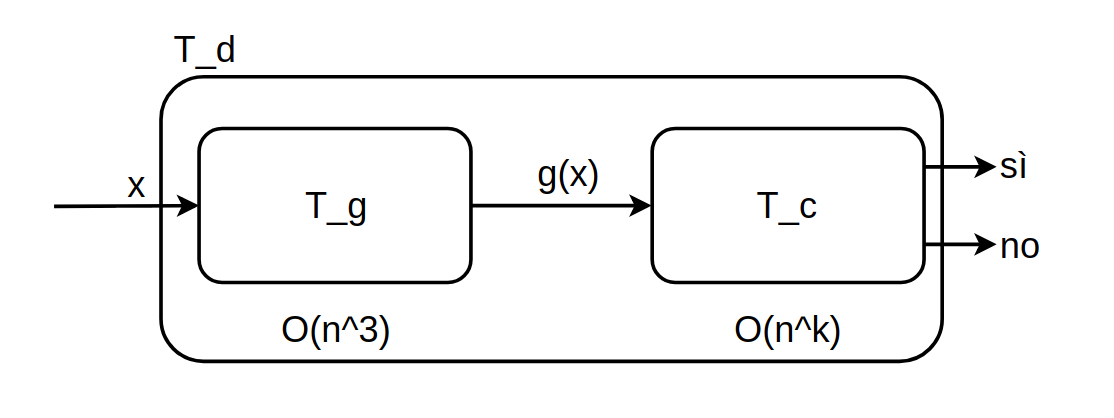
\includegraphics[width=\textwidth]{riduzione-esercizio}
\end{figure}

Sia $n = |x|$ la dimensione dell'input; poiché il tempo limita lo spazio, possiamo dire che $|g(x)| = O(n^k)$. Da ciò discende che $T_c$ riceverà input di dimensione $O(n^k)$, e quindi $t_{T_d}(n) = t_{T_g}(n) + t_{T_c}(n^k) = O(n^k) + O((n^k)^3) = O(n^k) + O(n^{3k}) = O(n^{3k})$. Concludiamo quindi che $D \in TIME(n^{3k})$.

\newtheorem*{exc2}{Esercizio 2}
\begin{exc2}
Correggere le seguenti affermazioni:
\end{exc2}
\begin{enumerate}
			\item per dimostrare che $X \in NP$-completo si deve dimostrare:
				\begin{description}
					\item \textit{1.} $X \in NP$,
					\item \textit{2.} $X \leq_p Y$ per un $Y \in NP$-completo.
				\end{description}
				In questa affermazione è sbagliato dire $X \leq_p Y$ per un $Y \in NP$-completo. $X$ è $NP$-completo se un problema $NP$-completo può essere ridotto ad esso, quindi va corretta con $Y \leq_p X$ per un $Y \in NP$-completo.
			
			\item Esiste un problema $NP$-completo che si risolve in tempo polinomiale deterministico ma questo non è vero per $SAT$.\\
			Se esistesse un problema $NP$-completo polinomiale allora tutti i problemi $NP$-completi si ridurrebbero a questo problema. Ma anche $SAT \in NP$-completo e quindi anche esso sarebbe riducibile a questo problema.
						
			\item $X \leq_p SAT \ \forall X \in NP$-hard\\
			L'affermazione non è vera in generale, poiché NP-hard è una classe più estesa di NP, e poiché SAT è NP-completo, l'affermazione è vera per gli $X \in NP$.
		\end{enumerate}


\newtheorem*{exc3}{Esercizio 3}
\begin{exc3}
Siano $INDSET, VC$ i seguenti linguaggi:
\begin{gather*}
	INDSET = \{\langle G,k \rangle  \ \mid  \ G \ \text{ha un indipendent set di k vertici}\} \\
	VC = \{\langle G, k \rangle  \ \mid  \ \text{esiste un vertex cover di k vertici per } G\}
\end{gather*}
Esibire una riduzione $INDSET \leq_p VC$, sapendo che $VC$ è $NP$-completo
\end{exc3}
Vogliamo esibire una riduzione $\langle G,k \rangle  \xmapsto{f} \langle G', k' \rangle $ tale che 
\[
	G \text{ ha un indipendent set di k vertici} \iff G' \text{ ha un vertex cover di k' vertici}
\]
La $f$ di riduzione costruisce una istanza $\langle G', k' \rangle$ con $G'=G$ e $k'=|V|-k$. Mostriamo che questa è una riduzione corretta:
\begin{gather*}
	A \subseteq V_G \text{ è un indipendent set di} \  k \ \text{vertici } \\
	\iff \\
	V_G-A \text{ è un vertex cover di } |V|-k \text{ vertici}
\end{gather*}
$\implies: \{u,w\} \in E$ allora certamente $u$ e $w$ non possono essere entrambi in $A$, quindi $u \in V-A$ oppure $w \in V-A$, allora per ogni arco uno degli estremi sta in $V-A$, che quindi è un vertex cover. Poiché $|A| = k$, $|V-A| = |V|-k$, quindi abbiamo dimostrato che $V-A$ è un vertex cover di $|V| - k$ vertici.
\\
$\impliedby: $ Supponiamo per assurdo che $V_G - A$ sia un vertex cover, e che $A$ non sia un independent set. Se $A$ non fosse un independent set, allora $\exists u, w \in A$ tali che $\{u, w\} \in E$. Ma allora l'arco $\{u, w\}$ sarebbe "scoperto", in quanto nè $u$ nè $w$ stanno nel vertex cover, quindi $V_G - A$ non sarebbe un vertex cover (assurdo).